\documentclass[10pt]{article}
\usepackage{ucs}
\usepackage[a4paper, total={6in, 10in}]{geometry}
\usepackage[utf8x]{inputenc}
\usepackage{graphicx}
\title{Essential Skills: Statistics optional}
\date{5 October 2016}
\author{Ali Abdulmadzhidov}

\begin{document}
\renewcommand*\rmdefault{cmss}
\maketitle

\section{Examining Data}
\begin{enumerate}
    \item Load data and get total number of observations
        \begin{verbatim}
            > data(islands)
            > length(islands)
            [1] 48
        \end{verbatim}
    \item Mean and median
        \begin{verbatim}
            > mean(islands)
            [1] 1252.729
            > median(islands)
            [1] 41
        \end{verbatim}
    \item Size of smallest and biggest island
        \begin{verbatim}
            > range(islands)[1]
            [1] 12
            > range(islands)[2]
            [1] 16988
        \end{verbatim}
    \item Standart deviation and the range of the islands size using range
        \begin{verbatim}
            > sd(islands)
            [1] 3371.146
            > range(islands)[2] - range(islands)[1]
            [1] 16976
        \end{verbatim}
    \item Quantiles
        \begin{verbatim}
            > quantile(islands)
                   0%      25%      50%      75%     100% 
                12.00    20.50    41.00   183.25 16988.00
            > quantile(islands, c(.05,.95))
                  5%     95% 
               13.00 8481.75
        \end{verbatim}
    \item Interquartile range
        \begin{verbatim}
            > IQR(islands)
            [1] 162.75
        \end{verbatim}
    \item Histogram showing frequency and proportion of each group
        \begin{verbatim}
            > hist(islands)
        \end{verbatim}
        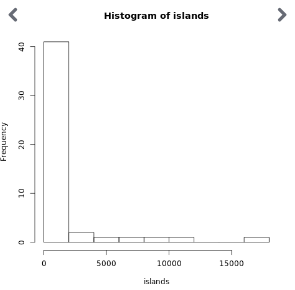
\includegraphics[scale=0.5]{hist1} \\ \\
        \begin{verbatim}
            > hist(islands, prob=T)
        \end{verbatim}
        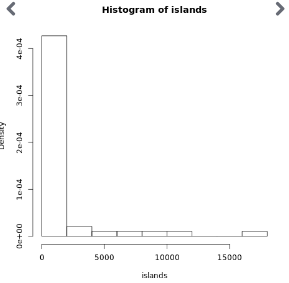
\includegraphics{hist2}
    \item Create box-plots with outliers and without them
        \begin{verbatim}
            > boxplot(islands)
        \end{verbatim}
        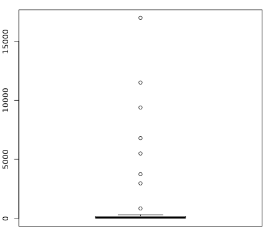
\includegraphics[scale=0.5]{boxplot} \\ \\
        \begin{verbatim}
            > boxplot(islands, outline = F)
        \end{verbatim} \\ \\
        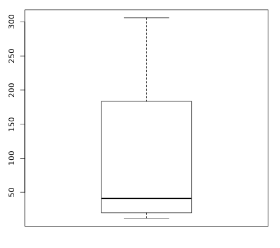
\includegraphics[scale=0.5]{boxplot2} \\ \\
    \item Using the function boxplot find the outliers of islands.
        \begin{verbatim}
            > boxplot(islands, plot=F)$out
               Africa    Antarctica          Asia     Australia        Europe 
                11506          5500         16988          2968          3745 
            Greenland North America South America 
                  840          9390          6795
        \end{verbatim}
    \item Create box-plots with the following conditions
        \begin{verbatim}
            stem(islands)
        \end{verbatim} \\ \\
    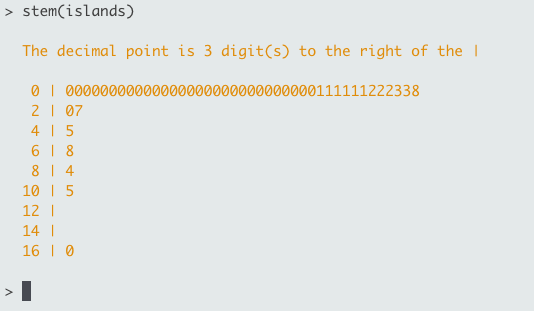
\includegraphics[scale=0.5]{stem}
\end{enumerate}



\section{Summary Statistics With Aggregate}
\begin{enumerate}
    \item Using R‘s built-in time series dataset, “AirPassengers“, compute the average annual standard deviation.
    \begin{verbatim}
    > aggregate(AirPassengers, nfrequency = 1, sd)
    Time Series:
    Start = 1949 
    End = 1960 
    Frequency = 1 
     [1] 13.72015 19.07084 18.43827 22.96638 28.46689 34.92449 42.14046 47.86178
     [9] 57.89090 64.53047 69.83010 77.73713
    \end{verbatim}
    \item Aggregate the “airquality” data by “airquality\$Month“, returning means on each of the numeric variables. Also, remove “NA” values.
        \begin{verbatim}
        > aggregate(airquality, list(airquality$Month), mean, na.rm=T)
          Group.1    Ozone  Solar.R      Wind     Temp Month  Day
        1       5 23.61538 181.2963 11.622581 65.54839     5 16.0
        2       6 29.44444 190.1667 10.266667 79.10000     6 15.5
        3       7 59.11538 216.4839  8.941935 83.90323     7 16.0
        4       8 59.96154 171.8571  8.793548 83.96774     8 16.0
        5       9 31.44828 167.4333 10.180000 76.90000     9 15.5
        \end{verbatim}
    \item Aggregate the “airquality” data by the variable “Day“, remove “NA” values, and return means on each of the numeric variables.
        \begin{verbatim}
        > aggregate(airquality, list(airquality$Day), mean, na.rm=T)
           Group.1    Ozone  Solar.R      Wind     Temp    Month Day
        1        1 77.75000 199.0000  6.780000 80.20000 7.000000   1
        2        2 43.00000 174.8000  9.160000 80.80000 7.000000   2
        3        3 33.25000 177.4000  9.620000 79.40000 7.000000   3
        4        4 62.33333 197.2500  8.620000 81.80000 7.000000   4
        5        5 48.66667 163.3333  8.460000 79.20000 7.000000   5
        6        6 41.50000 223.3333 12.040000 79.80000 7.000000   6
        7        7 54.20000 241.8000  7.660000 80.80000 7.000000   7
        8        8 57.00000 217.6000  9.520000 81.20000 7.000000   8
        9        9 61.40000 203.8000 11.700000 81.60000 7.000000   9
        10      10 49.33333 234.6000  9.160000 82.00000 7.000000  10
        11      11 25.50000 192.7500 10.560000 83.20000 7.000000  11
        12      12 22.75000 244.2000 12.040000 79.20000 7.000000  12
        13      13 23.40000 224.8000  9.980000 77.60000 7.000000  13
        14      14 29.33333 215.6000 12.040000 78.00000 7.000000  14
        15      15 12.66667 122.2000 12.400000 73.40000 7.000000  15
        16      16 30.20000 218.6000 10.100000 75.40000 7.000000  16
        17      17 36.60000 228.0000 12.620000 73.20000 7.000000  17
        18      18 24.60000 108.4000 10.320000 71.60000 7.000000  18
        19      19 35.20000 222.2000  9.860000 74.80000 7.000000  19
        20      20 29.40000 158.4000  9.960000 76.60000 7.000000  20
        21      21 12.75000 132.4000 10.200000 70.20000 7.000000  21
        22      22 14.33333 137.4000 10.300000 74.60000 7.000000  22
        23      23 20.00000 161.0000  9.740000 75.00000 7.000000  23
        24      24 41.00000 179.4000  9.380000 74.20000 7.000000  24
        25      25 96.66667 136.4000 10.520000 72.20000 7.000000  25
        26      26 41.00000 176.4000  9.280000 74.80000 7.000000  26
        27      27 52.00000 106.7500  9.840000 76.20000 7.000000  27
        28      28 48.75000 143.6000 10.980000 81.40000 7.000000  28
        29      29 57.75000 182.8000  9.500000 82.80000 7.000000  29
        30      30 70.75000 214.8000  7.780000 81.80000 7.000000  30
        31      31 60.33333 240.3333  7.633333 83.66667 6.666667  31
        \end{verbatim}
    \item Aggregate “airquality\$Solar.R” by “Month“, returning means of “Solar.R“. The header of column 1 should be “Month“. Remove “not available” values.
        \begin{verbatim}
        > aggregate(airquality$Solar.R, list(Month=airquality$Month), mean, na.rm=T)
          Month        x
        1     5 181.2963
        2     6 190.1667
        3     7 216.4839
        4     8 171.8571
        5     9 167.4333
        \end{verbatim}
    \item Apply the standard deviation function to the data aggregation from Exercise
        \begin{verbatim}
        > aggregate(airquality$Solar.R, list(Month=airquality$Month), sd, na.rm=T)
          Month         x
        1     5 115.07550
        2     6  92.88298
        3     7  80.56834
        4     8  76.83494
        5     9  79.11828
        \end{verbatim}
    \item Use aggregate.formula for a oneto-one aggregation of “airquality” by the mean of “Ozone” to the grouping variable “Day“.
        \begin{verbatim}
        > aggregate(Ozone ~ Day, airquality, mean)
           Day    Ozone
        1    1 77.75000
        2    2 43.00000
        3    3 33.25000
        4    4 62.33333
        5    5 48.66667
        6    6 41.50000
        7    7 54.20000
        8    8 57.00000
        9    9 61.40000
        10  10 49.33333
        11  11 25.50000
        12  12 22.75000
        13  13 23.40000
        14  14 29.33333
        15  15 12.66667
        16  16 30.20000
        17  17 36.60000
        18  18 24.60000
        19  19 35.20000
        20  20 29.40000
        21  21 12.75000
        22  22 14.33333
        23  23 20.00000
        24  24 41.00000
        25  25 96.66667
        26  26 41.00000
        27  27 52.00000
        28  28 48.75000
        29  29 57.75000
        30  30 70.75000
        31  31 60.33333
        \end{verbatim}
    \item Use aggregate.formula for a many-to-one aggregation of “airquality” by the mean of “Solar.R” and “Ozone” by grouping variable, “Month“.
        \begin{verbatim}
        > aggregate(cbind(Solar.R, Ozone) ~ Month, airquality, mean)
          Month  Solar.R    Ozone
        1     5 182.0417 24.12500
        2     6 184.2222 29.44444
        3     7 216.4231 59.11538
        4     8 173.0870 60.00000
        5     9 168.2069 31.44828
        \end{verbatim}
    \item Use “.” dot notation to find the means of the numeric variables in airquality“, with the grouping variable of “Month“
        \begin{verbatim}
        > aggregate(. ~ Month, airquality, mean)
          Month    Ozone  Solar.R      Wind     Temp      Day
        1     5 24.12500 182.0417 11.504167 66.45833 16.08333
        2     6 29.44444 184.2222 12.177778 78.22222 14.33333
        3     7 59.11538 216.4231  8.523077 83.88462 16.23077
        4     8 60.00000 173.0870  8.860870 83.69565 17.17391
        5     9 31.44828 168.2069 10.075862 76.89655 15.10345
        \end{verbatim}
    \item Use dot notation to find the means of the “airquality” variables, with the grouping variables of “Day” and “Month“. Display only the first 6 resulting observations.
        \begin{verbatim}
        > head(aggregate(. ~ Day + Month, airquality, mean))
          Day Month Ozone Solar.R Wind Temp
        1   1     5    41     190  7.4   67
        2   2     5    36     118  8.0   72
        3   3     5    12     149 12.6   74
        4   4     5    18     313 11.5   62
        5   7     5    23     299  8.6   65
        6   8     5    19      99 13.8   59
        \end{verbatim} \\ \\
    \item Use dot notation to find the means of “Temp“, with the remaining “airquality” variables as grouping variables.
        \begin{verbatim}
        > aggregate(Temp ~ ., airquality, mean)
            Ozone Solar.R Wind Month Day Temp
        1      41     190  7.4     5   1   67
        2     135     269  4.1     7   1   84
        3      39      83  6.9     8   1   81
        4      96     167  6.9     9   1   91
        5      36     118  8.0     5   2   72
        6      49     248  9.2     7   2   85
        7       9      24 13.8     8   2   81
        8      78     197  5.1     9   2   92
        9      12     149 12.6     5   3   74
        10     32     236  9.2     7   3   81
        11     16      77  7.4     8   3   82
        12     73     183  2.8     9   3   93
        13     18     313 11.5     5   4   62
        14     91     189  4.6     9   4   93
        15     64     175  4.6     7   5   83
        16     47      95  7.4     9   5   87
        17     40     314 10.9     7   6   83
        18     32      92 15.5     9   6   84
        19     23     299  8.6     5   7   65
        20     29     127  9.7     6   7   82
        21     77     276  5.1     7   7   88
        22    122     255  4.0     8   7   89
        23     20     252 10.9     9   7   80
        24     19      99 13.8     5   8   59
        25     97     267  6.3     7   8   92
        26     89     229 10.3     8   8   90
        27     23     220 10.3     9   8   78
        28      8      19 20.1     5   9   61
        29     71     291 13.8     6   9   90
        30     97     272  5.7     7   9   92
        31    110     207  8.0     8   9   90
        32     21     230 10.9     9   9   75
        33     39     323 11.5     6  10   87
        34     85     175  7.4     7  10   89
        35     24     259  9.7     9  10   73
        36     44     236 14.9     9  11   81
        37     16     256  9.7     5  12   69
        38     10     264 14.3     7  12   73
        39     44     192 11.5     8  12   86
        40     21     259 15.5     9  12   76
        41     11     290  9.2     5  13   66
        42     23     148  8.0     6  13   82
        43     27     175 14.9     7  13   81
        44     28     273 11.5     8  13   82
        45     28     238  6.3     9  13   77
        46     14     274 10.9     5  14   68
        47     65     157  9.7     8  14   80
        48      9      24 10.9     9  14   71
        49     18      65 13.2     5  15   58
        50      7      48 14.3     7  15   80
        51     13     112 11.5     9  15   71
        52     14     334 11.5     5  16   64
        53     21     191 14.9     6  16   77
        54     48     260  6.9     7  16   81
        55     22      71 10.3     8  16   77
        56     46     237  6.9     9  16   78
        57     34     307 12.0     5  17   66
        58     37     284 20.7     6  17   72
        59     35     274 10.3     7  17   82
        60     59      51  6.3     8  17   79
        61     18     224 13.8     9  17   67
        62      6      78 18.4     5  18   57
        63     20      37  9.2     6  18   65
        64     61     285  6.3     7  18   84
        65     23     115  7.4     8  18   76
        66     13      27 10.3     9  18   76
        67     30     322 11.5     5  19   68
        68     12     120 11.5     6  19   73
        69     79     187  5.1     7  19   87
        70     31     244 10.9     8  19   78
        71     24     238 10.3     9  19   68
        72     11      44  9.7     5  20   62
        73     13     137 10.3     6  20   76
        74     63     220 11.5     7  20   85
        75     44     190 10.3     8  20   78
        76     16     201  8.0     9  20   82
        77      1       8  9.7     5  21   59
        78     16       7  6.9     7  21   74
        79     21     259 15.5     8  21   77
        80     13     238 12.6     9  21   64
        81     11     320 16.6     5  22   73
        82      9      36 14.3     8  22   72
        83     23      14  9.2     9  22   71
        84      4      25  9.7     5  23   61
        85     36     139 10.3     9  23   81
        86     32      92 12.0     5  24   61
        87     80     294  8.6     7  24   86
        88     45     212  9.7     8  24   79
        89      7      49 10.3     9  24   69
        90    108     223  8.0     7  25   85
        91    168     238  3.4     8  25   81
        92     14      20 16.6     9  25   63
        93     20      81  8.6     7  26   82
        94     73     215  8.0     8  26   86
        95     30     193  6.9     9  26   70
        96     52      82 12.0     7  27   86
        97     23      13 12.0     5  28   67
        98     82     213  7.4     7  28   88
        99     76     203  9.7     8  28   97
        100    14     191 14.3     9  28   75
        101    45     252 14.9     5  29   81
        102    50     275  7.4     7  29   86
        103   118     225  2.3     8  29   94
        104    18     131  8.0     9  29   76
        105   115     223  5.7     5  30   79
        106    64     253  7.4     7  30   83
        107    84     237  6.3     8  30   96
        108    20     223 11.5     9  30   68
        109    37     279  7.4     5  31   76
        110    59     254  9.2     7  31   81
        111    85     188  6.3     8  31   94
        \end{verbatim}
\end{enumerate}


\end{document}